\section{Aufgabenstellung}
Beim Programmierwettbewerb für das Freie Magazin ging es diesmal um einen
Tagcloud-Generator. 
Dabei sollten einige Anforderungen erfüllt werden:
\begin{itemize}
    \item rein textuelle Analyse
    \item Eingabe von Trennzeichen
    \item rekursive Suche und Analyse von Dateien mit
        bestimmten Dateiendungen
    \item Angabe von mindestens einer Liste mit Wörtern, die ignoriert werden sollen
    \item Angabe von mindestens einer Liste mit Wörtern oder Wortzusammensetzungen, die speziell gezählt werden sollen (A)
    \item Einstellbarkeit für die Anzahl der sichtbaren Wörter in der Wortwolke
    \item Einstellbarkeit für die minimal zu beachtende Wortlänge
    \item Darstellung als Wortwolke
\end{itemize}
Die Anforderung(A) wurde bisher noch nicht umgesetzt, alle anderen sind implementiert.
\section{Lösung/Aufbau}
Der hier beschriebene Tagcloud-Generator namens 'Cloudtag' wurde in Python3 implementiert und benutzt nur die
Standartpython Bibliotheken.


Er besteht aus mehreren Python3 Modulen:
\begin{description}
    \item ~
     \begin{description}
            \item[ctlib.py] einige Funktionen die von allen Modulen benutzt werden
            \item[ct.py] einfaches all-one Skript
            \item[ctana.py] Textanalyse
            \item[ctmerge.py] Zusammenfügen von mehreren Textdateien in rekursiven Unterverzeichnissen
            \item[ctsimple.py] einfache html basierte Ausgabe
            \item[ctspiral.py] svg basierte Wolken-Ausgabe, benutzt Spiralen
        \end{description}
\end{description}


Im ausgelieferten Paket findet man folgende Ordnerstruktur vor:
\begin{itemize}
    \item cfg : Konfigurationsverzeichnis
        \begin{itemize}
            \item ignore 
                \begin{itemize}
                    \item chars.txt : Zeichen die ignoriert werden sollen 
                    \item words.txt : Wörter die ignoriert werden
                \end{itemize}
            \item pattern
                \begin{itemize}
                    \item html.pat : html Vorlage
                    \item svg.pat : svg Vorlage
                \end{itemize}
            \item config.cfg : allgemeine Konfigurationsdatei
        \end{itemize}
    \item in : Beispieltexte  
    \item out : Beispielausgabe
    \item doc : dieses Dokument
\end{itemize}

\section{Konfiguration}
Alle Module benutzen die gleichen Konfigurationsdatein aus dem Verzeichnis 'cfg'.
Die 'ignore' Dateien haben dabei einen einfachen Aufbau, denn in jeder Zeile steht genau ein Wort bzw. ein Zeichen 
welches ignoriert werden soll.

Die wichtigste Konfigurationsdatei ist 'config.cfg'. Man kann Farben, Schriftgröße, die Dateien zum Ignorieren, verschiedene Vorlagen zur Ausgabe 
und andere Parameter anpassen.
Sie sieht beispielsweise folgendermaßen aus:
\lstset{tabsize=4,basicstyle=\footnotesize\ttfamily,stringstyle=\color{Orange},showstringspaces=false,columns=fixed}
\begin{lstlisting}
[ignore] #ignore settings
# base directory for ignore lists
base = cfg/ignore/
# ignore lower / uppercase
case = True
# textfilename for ignored word list
words = words.txt
# textfilename for ignored char list
chars = chars.txt
[words] # tag cloud settings
# maximal words=-1 means use all words
max = -1
# maximal frequency of words
maxfreq = -1
# minimal frequency of words
minfreq = 10
# minimal length of words
minlen = 3
[font] # font size in pixel
max = 90
min = 14
[color]
min = 00FF00
max = FF0000
[pattern]
base = cfg/pattern/
# delimiter
split = #
# html pattern file
html= html.pat
# svg pattern
svg= svg.pat
[output]# outputformats 
format = html,svg
\end{lstlisting}
Die Parameter sind soweit selbsterklärend
\section{Benutzung}
\subsection{einfach}
Die einfachste Möglichkeit bietet die Benutzung von 'ct.py'.
\\
Ein './ct.py -h' zeigt Informationen zu den Parametern.
\subsection*{minimale Parameter}
'ct.py' benötigt mindestens 2 Parameter, einmal 'in' und dann noch 'outfilebase':
\begin{description}
      \item['in'] wobei 'in' die Eingabedatei oder das Eingabeverzeichnis ist und
      \item['outfilebase']der Basisname (bzw. Pfad und Basisname) für die Ausgabedateien ist.
\end{description}
Möchte man z.b. nur eine Html Ausgabe, so muss man in der 'config.cfg'
unter 'output' den Parameter 'format' auf 'format=html' setzen. 
Nach Aufruf von 'ct.py in outfilebase' werden dann die Dateien 'outfilebase'.plain und 'outfilebase'.html angelegt.
Die '*.plain' Dateien beinhalten dabei das Ergebnis der Textanalyse in einfacher Form. 

\subsection{anderes Vorgehen}
Man muss nicht jedes mal eine erneute Textanalyse durchführen, oder jedes mal die Eingabe Dateien zusammenfügen,
sondern man kann jeden einzelnen Schritt der bei 'ct.py' durchgeführt wird auch mit dem jeweiligen extra 'ctX' Tool durchführen.
Einfach das jeweilige Programm ohne Parameter starten und man erhält Informationen über die Parameter.

\clearpage
\section{Technik/Tests}
Mit dem Script 'test.sh' werden Dateien die im Verzeichnis 'in' unterschiedlich als TagClouds verarbeitet und 
im Verzeichnis 'out' gespeichert.
Zum Beispiel sollte dabei eine Tag-Cloud zu 'Faust' erzeugt werden:
\begin{center}
    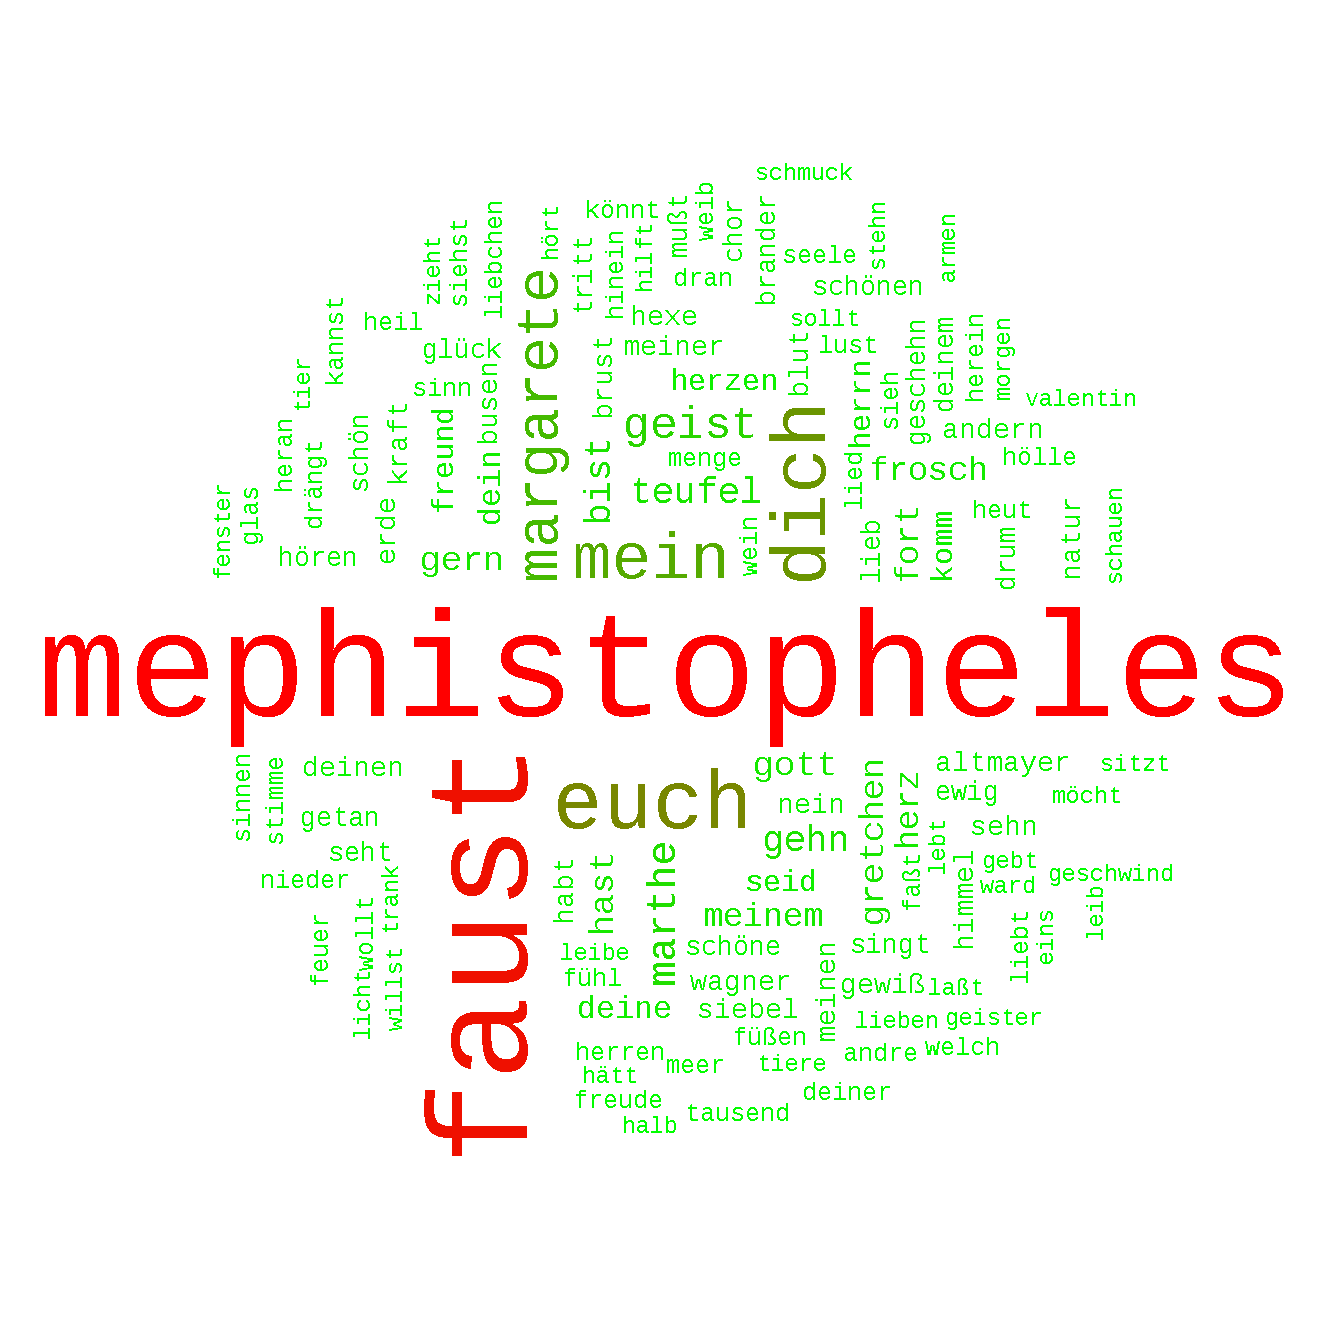
\includegraphics[width=0.8\textwidth]{images/faust.pdf}    
\end{center}
Am Anfang werden alle Wörter zufällig in einem Kreis ausgerichtet (das häufigste Wort in der Mitte),
anschließend wird in absteigender Häufigkeit getestet, ob sich das Wort mit einem bereist gespeicherten überschneidet.
Tritt dieser Fall ein (was fast immer passiert), wird entlang eine Spirale (siehe Abbildung) eine Position ohne Überschneiden gefunden.
\begin{center}
    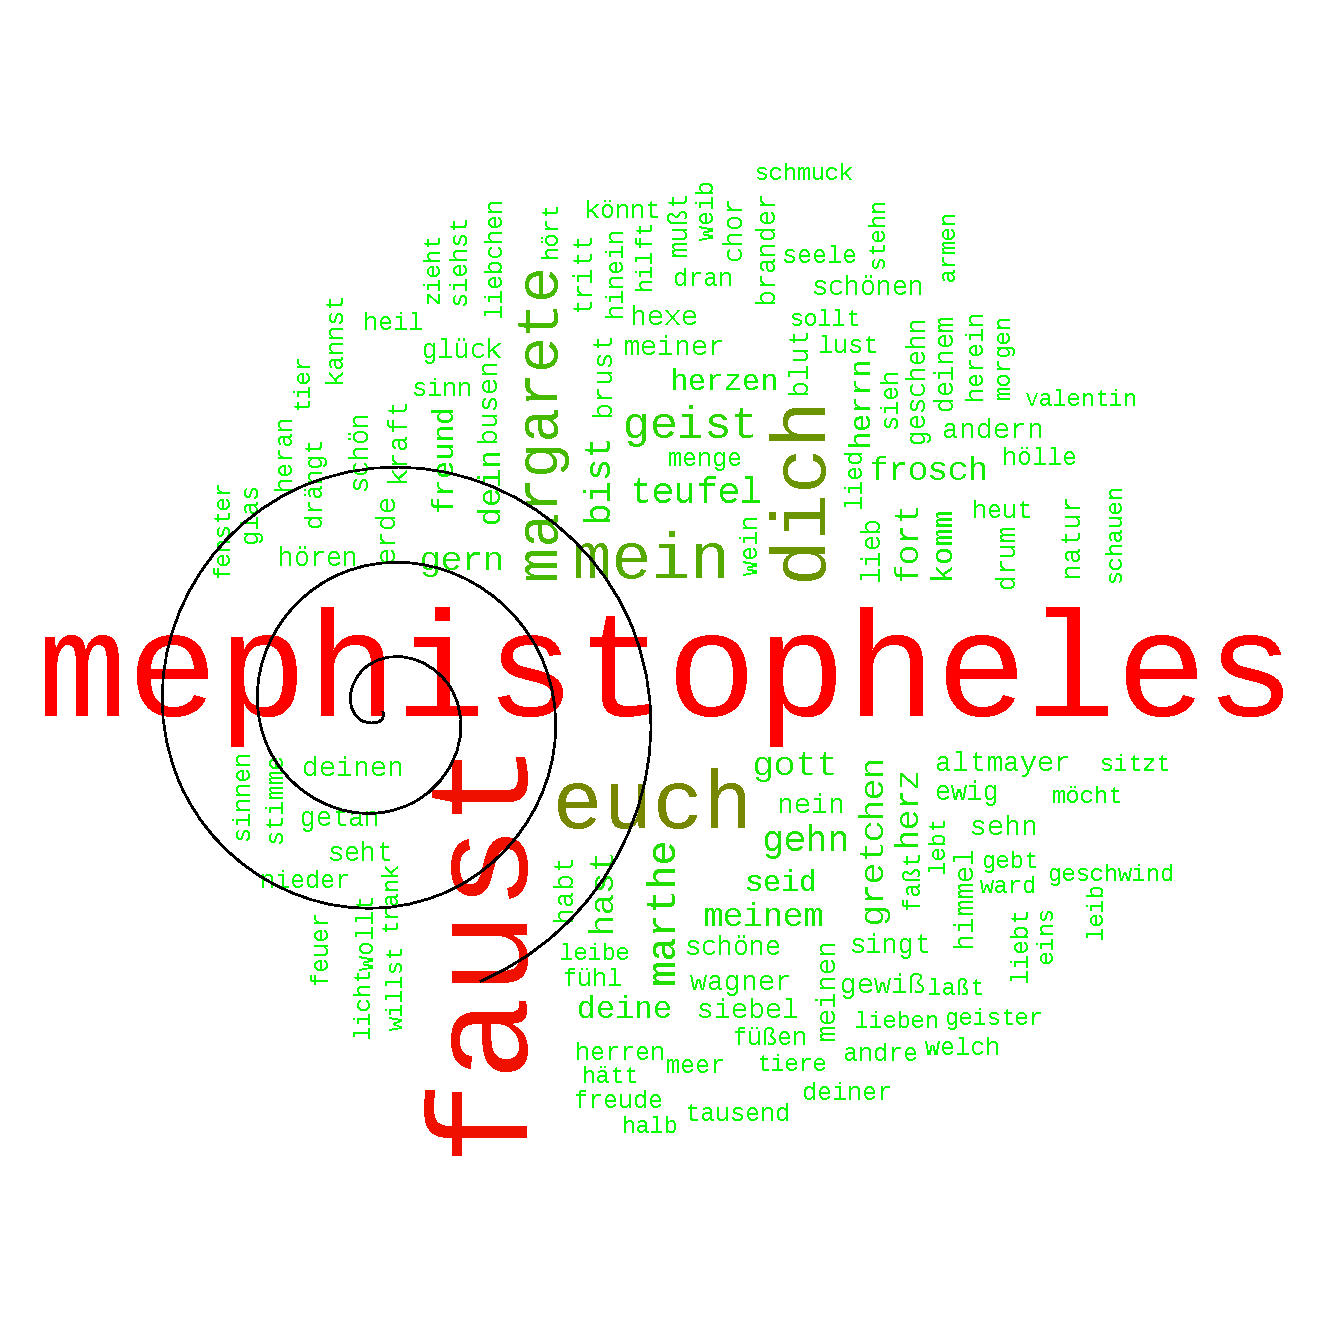
\includegraphics[width=0.8\textwidth]{images/faust2.pdf}    
\end{center}
Problematisch an der Vorgehensweise sind die ständigen Kollisionstests zwischen Wörtern (die als Rechtecke behandelt werden),
in der Implementierung wird dabei noch ein recht einfaches Durchtesten benutzt, besser wäre hier der Einsatz eines 
Quadtrees oder R-Trees.

\section{Offen}
Z.b. die Anforderung (A), zusätzliche Anforderungen (Kommentare ignorieren,...), bessere Kollisionstests.
Andere Ausgabe'plugins', z.B. gravitationsbasierend, sternförmig, hierarchisch.
Während der Tests in der Entwicklung wurde auch probiert ein 3 GB Wikipedia Dump File zu analysieren,
das ist aber leider nur mit ausreichend Hauptspeicher möglich, diese Problem könnte man Lösen 
in dem man die Eingabedatei, falls sie größer als irgendeine Grenze, stückchenweise analysiert und die Hisotgramme 
der einzelnen Analysen dann zusammenfügt.


